\documentclass[
a4paper,   
headsepline, 
fleqn,     
11pt
]{scrartcl}

%%% ngerman: language set to new-german
\usepackage{ngerman}
\usepackage[latin1]{inputenc}
\usepackage[T1]{fontenc}
\usepackage{ae,aecompl}

%%% Graphic stuff
\usepackage{graphicx}
\usepackage{geometry}
\geometry{verbose,a4paper,tmargin=25mm,bmargin=25mm,lmargin=15mm,rmargin=20mm}
\usepackage{amsmath,amssymb,amstext}
\usepackage{units}
\usepackage{scrpage2}

%%% comments, ...
\usepackage{verbatim}

\setlength{\parindent}{0em} 

\newcommand{\mygraphics}[3]{
  \begin{center}
    \includegraphics[width=#1, keepaspectratio=true]{#2} \\
    \textbf{#3}
  \end{center}
}

%%%      footer - middle: page number
\pagestyle{scrheadings}

%%% heading - left
 \ihead[]{Marco Sohm, Kevin Wallis}

%%% heading - right
 \ohead[]{Aufgabe 2}

\begin{document}

 \pagenumbering{roman} %% small roman page numbers
 \pagenumbering{arabic} 

\subsection*{Einleitende Worte}
Die Einheit f�r die Arbeit wurde in Stunden definiert. Alle im Model verwendeten Funktionen (Table Functions) sind in Prozent angegeben und mit dem Leistungsumrechnungfaktor verbunden. So bedeutet beispielsweise $Integrationsverluste\_MIE(MitarbeiterInEinarbeitung)$ f�r $Argument = 2$ und $Value = 12,5$ (Einheit \%), dass bei zwei Mitarbeitern in Einarbeitung eine Stunde (= 0,125 * 8) pro Tag f�r die Integration eingeplant werden muss.

\subsection*{zu a) Ideen hinter der Modellierung}
\begin{comment}
a) Versuchen Sie, das Modell soweit zu bringen, da� plausible Simulationsresultate zu beobachten sind. Falls Sie dazu selbst�ndig Information in das Modell hineingebracht haben, die nicht im Buchkapitel angegeben wurden, begr�nden Sie Ihre Wahl mit vollst�ndigen S�tzen. Suchen Sie auch danach, wo sinnvollerweise realistische Reaktionszeiten einzubauen sind. Bauen Sie sie dann ein und beobachten Sie das Resultat.
\end{comment}
Folgende Beschreibung ist nicht vollst�ndig, sondern beschr�nkt sich haupts�chlich auf Abweichungen bzw. Erweiterungen zu 'Der Termin'. \\

\textbf{Parameter}: \\
\textbf{Leistungsumrechnungfaktor}: Wird verwendet um ein Ma� f�r die Arbeit zu definieren. Der Standardwert betr�gt acht und bedeutet, dass pro Tag (Model Zeiteinheit) maximal bis zu acht Stunden pro Mitarbeiter verrichtet werden k�nnen.
\textbf{Leistungsfaktor\_VM}: Standard 0.9. Bedeutet, dass ein verf�gbarer Mitarbeiter 90\% seiner Arbeitszeit f�r die Abarbeitung der offenen Arbeit verwendet. 
\textbf{Leistungsfaktor\_MIE}: Standard 0.2. Analog zu Leistungsfaktor\_VM.

\textbf{Dynamische Variablen}: \\
\textbf{Integrationskosten}: 
Die Integrationskosten sind abh�ngig von den Mitarbeitern in Einarbeitung aber auch von den verf�gbaren Mitarbeitern. Je mehr Mitarbeiter in Einarbeitung desto gr��er die Kosten. Kompensiert werden k�nnen diese Kosten durch die verf�gbaren Mitarbeiter. Modelliert durch: 
$Integrationsverluste\_MIE(MitarbeiterInEinarbeitung)$ \\ $- Integrationsgewinn\_VM(VerfuegbareMitarbeiter)$ (Umrechnungsfaktoren vernachl�ssigt) \\
\textbf{Interaktionsverlust}:
Modelliert durch: \\
$InteraktionsverlustFunktion(VerfuegbareMitarbeiter) / Teamdynamik$ \\
Interaktion findet auch bei Mitarbeitern in Einarbeitung statt. Diese wird jedoch in den Integrationsverlust einbezogen.
\textbf{Teamdynamik}:
Die Teamdynamik ist als Funktion der Fluktuation, Integration und verf�gbaren Mitarbeiter modelliert. Dabei wird eine Funktion verwendet, die der Fluktuation und Integration auch noch eine Abh�ngigkeit der Zeit zuordnet. Damit wird erreicht, dass eine sich stark �ndernde Fluktuation bzw. Integration keine sofortige 100 prozentige Auswirkung auf die Teamdynamik hat. Die Abbildung erfolgt dabei linear und nach einer einmonatigen konstanten Rate werden die 100\% erreicht.
Es findet au�erdem ein Mapping statt, dass die berechneten Werte auf den Bereich 0.5-2 einschr�nkt, weil die Teamdynamik bei den Interaktionsverlusten im Nenner steht. Schlechte Teamdynamik k�nnte damit auch zu erh�hten Interaktionsverlusten f�hren bzw. maximal um den Faktor zwei halbieren.
\textbf{MIE}: Die Summe der Arbeit in Stunden die von allen Mitarbeitern in Einf�hrung pro Tag verrichtet wird.
\textbf{VM}: Analog zu MIE.

\textbf{Delays}: \\
Es wurde ein Delay eingef�hrt, dass nicht sofort nach der K�ndigung eines Mitarbeiters ein neuer Mitarbeiter eingef�hrt wird (Einstellungsverz�gerung).


\subsection*{zu b) Variation der Integration und Teamdynamik}
\begin{comment}
b) Variieren Sie Integrationszeit (also die entsprechende Rate),und die Wirkung der Teamdynamik in einem sinnvollen Bereich, und beschreiben Sie verbal und mit einem Graphen/Plot die beobachteten Ver�nderungen im System. Geben Sie einen Erkl�rungsversuch.
\end{comment}

Die vorgenommen Simulationsergebnisse wurden im Anhang als Grafiken beigef�gt (Abbildung: \ref{fig:Model_Seite_16}, \ref{fig:Model_Seite_16_EZ30} und  \ref{fig:Model_Seite_16_EZ30_Td10}). Aus diesen Simulationen kann abgeleitet werden, das wenn die Einarbeitungszeit kleiner wird die komplette offene Arbeit schneller erledigt wird. Wenn die Einarbeitungszeit gr��er wird, tritt das Gegenteil ein und die offene Arbeit braucht l�nger bis sie erledigt ist. Somit besteht eine Auswirkung auf die Gesamtproduktionsleistung, bei gr��erer Einarbeitungszeit ist die Gesamtproduktionsleistung kleiner und vice versa. Bei einer kleineren Teamdynamik wird die Dauer f�r das Erledigen der kompletten Arbeit gr��er, dies entspricht auch der Intuitiven Vorstellung von uns.

\newpage

\subsection*{Anhang}
Die folgenden Diagramme stellen Vergleiche zu 'Der Termin' her. Dabei ist
darauf zu achten, dass Abweichungen zu den dort dargestellten Modellen bestehen. So wurde teilweise vereinfacht und/oder weitere Konzepte hinzugef�gt.

\begin{figure}[h]
  \centering
  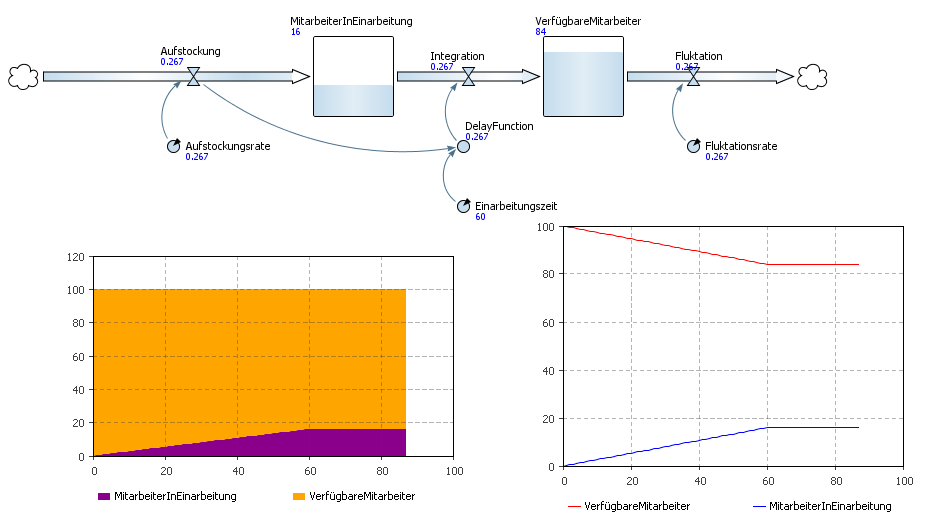
\includegraphics[width=1\textwidth]{./images/Model1_Seite8}
  \caption{Model Stage 1 (vergleiche Seite 8 'Der Termin')}
  \label{fig:Model_Seite_8}
\end{figure}

\begin{figure}[h]
  \centering
  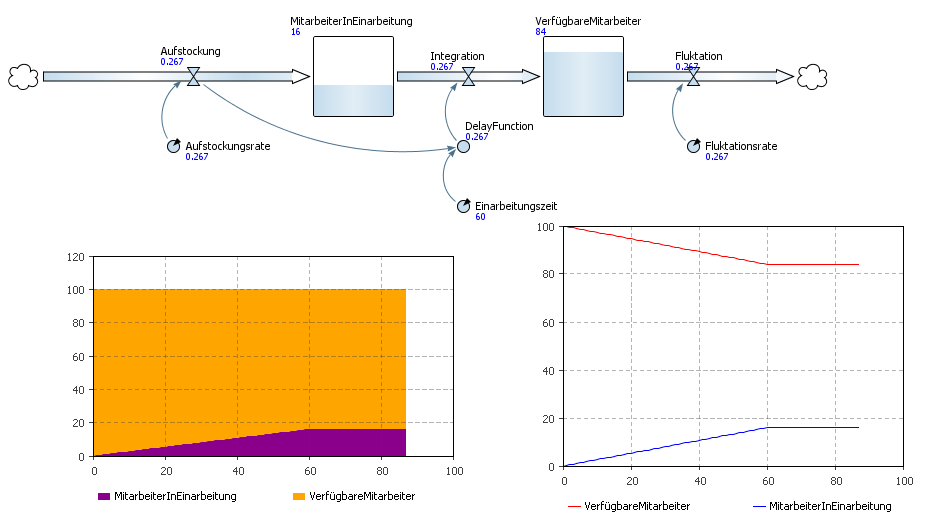
\includegraphics[width=1\textwidth]{./images/Model1_Seite16}
  \caption{Ergebnis des erweiterten Models (vergleiche Seite 16 'Der Termin')}
  \label{fig:Model_Seite_16}
\end{figure}

\begin{figure}[h]
  \centering
  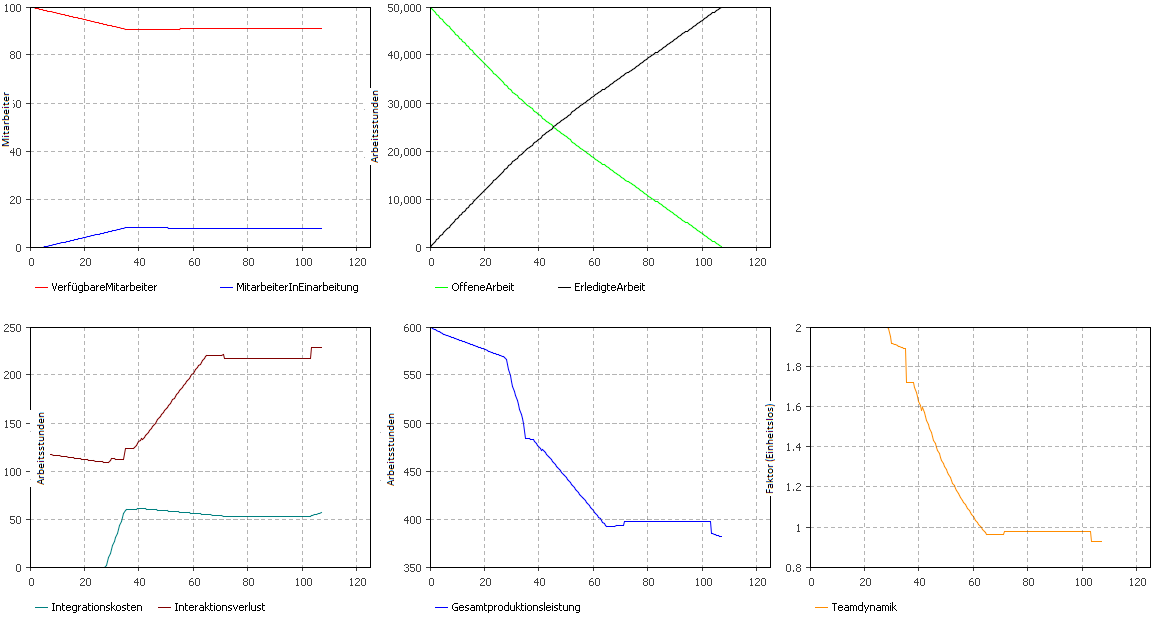
\includegraphics[width=1\textwidth]{./images/Model1_Seite16_Einarbeitungszeit30}
  \caption{Einarbeitungszeit 30 (statt 60)}
  \label{fig:Model_Seite_16_EZ30}
\end{figure}

\begin{figure}[h]
  \centering
  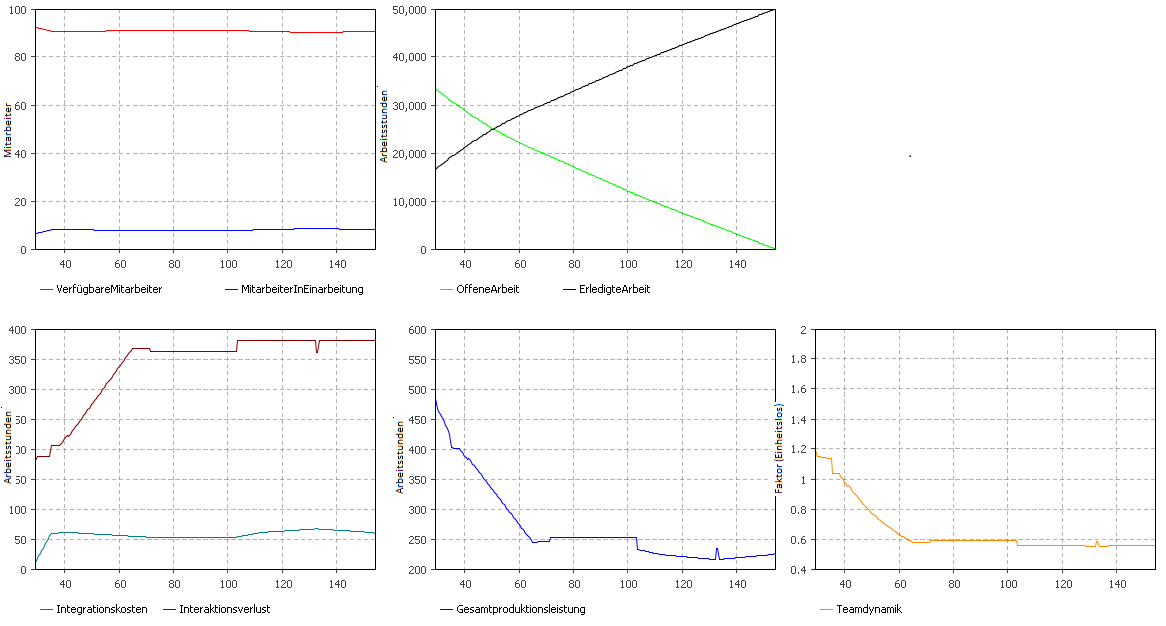
\includegraphics[width=1\textwidth]{./images/Model1_Seite16_Einarbeitungszeit30_TeamDynInfluenceFactor10}
  \caption{Einarbeitungszeit 30 (statt 60) und kleinerem Einfluss der Teamdynamik}
  \label{fig:Model_Seite_16_EZ30_Td10}
\end{figure}



\appendix  
\bibliographystyle{plain}
\bibliography{projekt.bib}

\end{document}